% !TeX spellcheck = en_US
\chapter{Challenges and Open Problems}

\section{References}
\begin{itemize}
	\item Deep \ac{RL} Doesn't Work Yet \cite{irpan18}
	\item \href{http://rail.eecs.berkeley.edu/deeprlcourse/static/slides/lec-23.pdf}{CS 285 at UC Berkeley, Deep \ac{RL}}
	\item Reproducible, Reusable, and Robust \ac{RL} \cite{pineau2018reproducible}
\end{itemize}
Multi-task transfer learning: deeper explanation for gradient interference and winner-take-all problem

\section{Reproducibility}
Checklist \cite{pineau2018reproducible}:

For all \textbf{algorithms} presented, check if you include:
\begin{todolist}
	\item A clear description of the algorithm.
	\item An analysis of the complexity (time, space, sample size) of the algorithm.
	\item A link to downloadable source code, including all dependencies.
\end{todolist}

For any \textbf{theoretical claim}, check if you include:
\begin{todolist}
	\item A statement of the result.
	\item A clear explanation of any assumptions.
	\item A complete proof of the claim.
\end{todolist}

For all \textbf{figures and tables} that present empirical results, check if you include:
\begin{todolist}
	\item A complete description of the data collection process, including sample size.
	\item A link to downloadable version of the dataset or simulation environment.
	\item An explanation of how sample were allocated for training / validation / testing.
	\item An explanation of any data that was excluded.
	\item The range of hyper-parameters considered, method to select the best hyper-parameter configuration, and specification of all hyper-parameters used to generate results.
	\item The exact number of evaluation runs.
	\item A description of how experiments were run.
	\item A clear definition of the specific measure or statistics used to report results.
	\item Clearly defined error bars.
	\item A description of results including central tendency (e.g. mean) and variation (e.g. stddev).
	\item The computing infrastructure used.
\end{todolist}


\section{Stability}
\subsection{Problem}
\begin{itemize}
	\item Devising stable RL algorithms is very hard
	\item Q-learning/value function estimation
	\begin{itemize}
		\item Fitted Q/fitted value methods with deep network function estimators are typically not contractions, hence no guarantee of convergence
		\item Lots of parameters for stability: target network delay, replay buffer size, clipping, sensitivity to learning rates, etc.
	\end{itemize}	
	\item Policy gradient/likelihood ratio/REINFORCE
	\begin{itemize}
		\item Very high variance gradient estimator
		\item Lots of samples, complex baselines, etc.
		\item Parameters: batch size, learning rate, design of baseline
	\end{itemize}	
	\item Model-based RL algorithms
	\begin{itemize}
		\item Model class and fitting method
		\item Optimizing policy w.r.t. model non-trivial due to back-propagation
		\item More subtle issue: policy tends to exploit the model
	\end{itemize}
	\item How representative is your simulator? Usually the answer is "not very"
\end{itemize}
\subsection{Directions}
Can we develop more stable algorithms that are less sensitive to hyperparameters?
\begin{itemize}
	\item Algorithms with favorable improvement and convergence properties
	\begin{itemize}
		\item Trust region policy optimization \cite{schulman2015icml}
		\item Safe \ac{RL}, high-confidence policy improvement
	\end{itemize}
	\item Algorithms that adaptively adjust parameters
	\begin{itemize}
		\item Q-Prop: Sample-efficient policy gradient with an off-policy critic \cite{gu2016q}
	\end{itemize}
\end{itemize}

\section{Sample Complexity}
\subsection{Problem}
Efficiency: how long does it take to converge? (how many samples)
\begin{itemize}
	\item Real-world learning becomes difficult or impractical
	\item Precludes the use of expensive, high-fidelity simulators
	\item Limits applicability to real-world problems
\end{itemize}
\cite{irpan18}

\subsection{Directions}
\begin{itemize}
	\item Better model-based \ac{RL} algorithms
	\item Design faster algorithms
	\begin{itemize}
		\item Addressing Function Approximation Error in Actor-Critic Algorithms \cite{fujimoto2018addressing}
		\item Soft Actor-Critic \cite{haarnoja2018soft}
	\end{itemize}
	\item Reuse prior knowledge to accelerate reinforcement learning
	\begin{itemize}
		\item RL2: Fast reinforcement learning via slow reinforcement learning \cite{duan2016rl}
		\item Learning to reinforcement learning \cite{wang2016learning}
		\item Model-agnostic meta-learning \cite{finn2017model}
		\item DREAM \cite{liu2020explore}
	\end{itemize}
\end{itemize}

\section{Scaling and Generalization}
Off-policy and Offline \ac{RL}

\section{Problem Formulation}
\subsection{Single Task or Multi-Task}
We have the assumption that the trained tasks and the test task are from the same distribution. As the result, with enough trials, the agent will visit every possible situations. But in real world, it's never like that.

Prior works on generalizing from multi-task learning:
\begin{itemize}
	\item Train on multiple tasks, then try to generalize or finetune
	\begin{itemize}
		\item Policy distillation \cite{rusu2015policy}
		\item Actor-mimic \cite{parisotto2015actor}
		\item Model-agnostic meta-learning \cite{finn2017model}
	\end{itemize}
	\item Unsupervised or weakly supervised learning of diverse behaviors
	\begin{itemize}
		\item Stochastic neural networks \cite{florensa2017stochastic}
		\item Reinforcement learning with deep energy-based policies \cite{haarnoja2017reinforcement}
		\item Unsupervised information-theoretic exploration
	\end{itemize}
\end{itemize}

\subsection{Supervision}
\begin{figure}[hbt!]
	\centering
	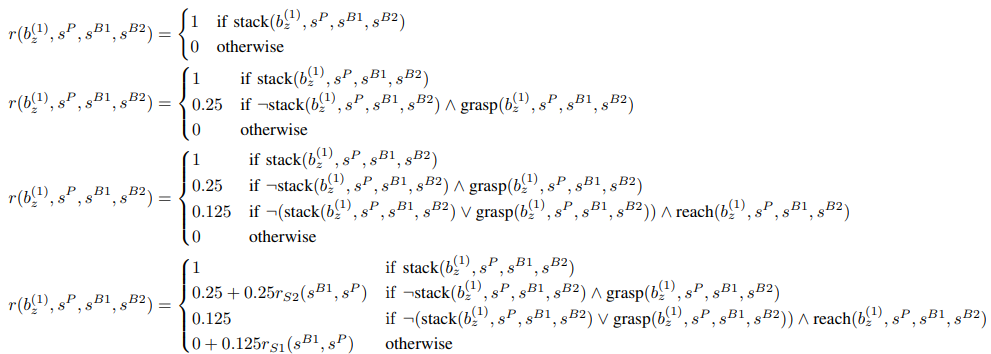
\includegraphics[width=\textwidth]{lego-stacking-reward.png}
	\caption{Complex reward function \cite{popov2017data}}
	\label{fig:lego-stacking-reward}
\end{figure}

\begin{itemize}
	\item If you want to learn from many different tasks, you need to get those tasks somewhere!
	\item Supervision comes from reward.
	\item Learn objectives/rewards from demonstration (inverse \ac{RL})
	\item Generate objectives automatically?
\end{itemize}

Unsupervised \ac{RL}
\begin{itemize}
	\item Interact with the world, without a reward function
	\item Learn something about the world (what?)
	\item Use what you learned to quickly solve new tasks
\end{itemize}